\documentclass[18pt,oneside,a4paper, titlepage]{article}

\usepackage[hidelinks]{hyperref}
\usepackage[pdftex]{graphicx}

\begin{document}
\begin{figure}[t]
	\centering
	
\includegraphics[scale=0.35]{logo-polimi.png}
\end{figure}
\title{\textbf{myTaxiService}\\\textbf{I}ntegration \textbf{T}est \textbf{P}lan \textbf{D}ocument\\ A.Y. 2015/2016\\
	Politecnico di Milano \\ Version 1.0}	
\author{Cattaneo Michela Gaia, matr. 791685\\Barlocco Mattia, matr. 792735 }
\date{January 22, 2016}
\maketitle

\newpage
	\tableofcontents

\newpage
\section{Introduction}
	\subsection{Revision History}
		% Record all revisions to the document.
	\subsection{Purpose	and	Scope}
		% State	the	purpose	and	scope of the document.
		\subsubsection{Purpose}
		This document represents the Integration Test Plan Document. It aims at specifying the plan for the integration testing of myTaxiService application, ensuring that all its modules interacts properly.\\
		This document is intended for the development team, that needs to know what it is needed to test, in which sequence it should occur and with which tools.
		\subsubsection{Scope}
		myTaxiService is an application that simplifies the access of the customers to the taxi service, managing also the taxi driver's distribution over the city and the queues of the areas. The customer can use the mobile application or the web app to request or reserve a taxi and a notification is forwarded to the designated taxi driver, who is going to answer.\\ This system should always be responsive and reliable, in order to keep up with all the requests of the passenger and the notifications forwarding.\\ This is the reason why the components that comprise the myTaxiService system are meant to be well integrated and tested.
	\subsection{List of	Definitions	and	Abbreviations}
		\begin{itemize}
			\item \textbf{Definitions}
			\item[-] \textbf{Passenger}: a person who is registered in the application.
			\item[-] \textbf{Taxi driver}: a taxi driver who access the application with a specific ID.
			\item[-] \textbf{Request}: the request of a taxi in a certain area and position in the city made by a user.
			\item[-] \textbf{Reservation}: the reservation of a taxi in a certain area, place and time that can be made only by passengers.
			\item[-] \textbf{Component}: a modular part of a system with encapsulated content and whose manifestation is replaceable within its environment.
			\item[-] \textbf{Subsystem}: a behavioral unit in the physical system, and hence in the model, and to serve as a specification unit for the behavior of its contained model elements.
						
			\item \textbf{Acronyms and abbreviations}
			\item[-] \textbf{RASD}: Requirement Analysis and Specification Document
			\item[-] \textbf{DD}: Design Document
			\item[-] \textbf{JEE}: Java Enterprise Edition
			\item[-] \textbf{JVM}: Java Virtual Machine
			
		\end{itemize}
	\subsection{List of	Reference Documents}
		%	List	all	reference	documents,	for	instance:
		%• The	project	description
		%• The	RASD
		%• The	Design	document
		%• The	documentation	of	any	tool	you	plan	to	use	for	testing
		\begin{itemize}
			\item Project Description and Rules (\url{https://github.com/MichelaCattaneo/myTaxiService/blob/master/Project\%20Description\%20And\%20Rules.pdf})
			\item Requirements Analysis and Specification Document (\url{https://github.com/MichelaCattaneo/myTaxiService/blob/master/Deliveries/RASD_1.1.pdf})
			\item Design Document (\url{https://github.com/MichelaCattaneo/myTaxiService/blob/master/Deliveries/DD.pdf})
			\item Integration Test Plan Example (\url{https://beep.metid.polimi.it/documents/3343933/5b3768d0-­‐‑d949-­‐‑4369-­‐‑87e1-­‐‑7a31b6943726})
		\end{itemize}

\newpage
\section{Integration Strategy}
	\subsection{Entry Criteria}	
		These are the criteria that must be respected before the integration testing phase may begin:
		\begin{itemize}
			\item Requirement Analysis and Specification Document is complete and revised
			\item Design Document is complete and revised
			\item Code Inspection Document is complete and revised
			\item The code is complete and high prioritized bugs fixed
			\item The product satisfies the requirements and the assumptions specified in the RASD
			\item The product satisfies the architecture and the design specified in the DD
			\item Test environment, test cases and test data are ready
		\end{itemize}	
		% Specify	the	criteria	that	must	be	met	before	integration testing of specific	elements	may	begin	(e.g.,	functions	must	have	been	unit tested).
	\subsection{Elements to	be Integrated}
		%Identify	the	components	to	be	integrated,	refer	to	your design	document	to	identify	such	components	in	a	way	that	is	consistent with	your	design.
		These components refer to the ones specified in the Component View in chapter 2.3 of the DD. This diagram shows how these components have to be integrated and the order of integration, according to the strategy adopted.
	\subsection{Integration Testing Strategy}
		% Describe	the	integration testing approach (top-down,	bottom-up,functional	groupings,	etc.)	and	the	rationale for	the	choosing that approach.
		The integration testing strategy that has been chosen exploits the bottom-up approach. This strategy is the most suitable for the myTaxiService system, in fact it makes it easier to find bugs, starting from the most critical components. The bottom-up approach starts from the lowest layers of the system, testing the basic functionalities at the beginning, then moving forward the most abstract layers, such as the client interfaces modules.\\ In this case, it is only necessary to use drivers, in order to simulate the top layers during the testing, which are a lot easier to produce with respect to the stubs used in the top-down approach.
	\newpage
	\subsection{Sequence of	Component/Function Integration}
		% NOTE:	 The structure	of	this	section	may	vary	depending	on	the	integration	strategy	you	select	in	Section	2.3. Use the structure proposed	below	as	a	non	mandatory	guide.	
		\subsubsection{Software	Integration	Sequence}
		% For	each	subsystem: Identify	the	sequence	in	which	the	software	components will	be	integrated within	the	subsystem.	Relate	this	sequence	to	any	product	features/functions	that	are	being	built	up.	
			In this section the system is presented already divided in the main three subsystems: Manager, Taxi Driver Client and Passenger Client.
			\begin{itemize}
				
				
				\item \textbf{Integration Test of the "Manager" subsystem }
					qui metteremo l'immagine
					\begin{center}
						\centering
						\begin{tabular}{c c c}
							\hline \textbf{ID} & \textbf{Integration Test} & \textbf{Paragraph} \\
							\hline		I1 & RequestManager $\rightarrow$ Database & \hyperlink{chapter 3.1}{3.1}\\
							\hline		I2 & PassengerAreaManager $\rightarrow$ Database & 3.2 \\
							\hline		I3 & TaxiDriverAreaManager $\rightarrow$ Database & 3.3\\
							\hline		I4 & AccessManager $\rightarrow$ Database & 3.4 \\
							\hline		I5 & RequestManager $\rightarrow$ PaymentManager & 3.5 \\
							\hline
						\end{tabular}
					\end{center}
				\item \textbf{Integration Test of the "Taxi Driver Client" subsystem }
					qui metteremo l'immagine
					\begin{center}
						\centering
						\begin{tabular}{c c c}
							\hline \textbf{ID} & \textbf{Integration Test} & \textbf{Paragraph} \\
							\hline		I6 & Notification $\rightarrow$ RequestManager & 3.6\\
							\hline		I7 & TaxiDriverArea $\rightarrow$ Notification & 3.7 \\
							\hline		I8 & TaxiDriverArea $\rightarrow$ TaxiDriverAreaManager & 3.8\\
							\hline		I9 & AccessManager $\rightarrow$ TaxiDriverArea & 3.9 \\
							\hline		I10 & Access $\rightarrow$ AccessManager & 3.10 \\
							\hline
						\end{tabular}
					\end{center}
				\item \textbf{Integration Test of the "Passenger Client" subsystem}
					qui metteremo l'immagine
					\begin{center}
						\centering
						\begin{tabular}{c c c}
							\hline \textbf{ID} & \textbf{Integration Test} & \textbf{Paragraph} \\
							\hline		I11 & ChoosePaymentMethod $\rightarrow$ PaymentManager & 3.11\\
							\hline		I12 & RequestManager $\rightarrow$ ChoosePaymentMethod & 3.12 \\
							\hline		I13 & MakeReservation $\rightarrow$ RequestManager & 3.13\\
							\hline		I14 & RequestTaxi $\rightarrow$ RequestMager & 3.14\\
							\hline		I15 & PassengerArea $\rightarrow$ RequestTaxi & 3.15 \\
							\hline		I16 & PassengerArea $\rightarrow$ MakeReservation & 3.16 \\
							\hline		I17 & PassengerArea $\rightarrow$ PassengerAreaManager & 3.17\\
							\hline		I18 & AccessManager $\rightarrow$ PassengerArea & 3.18 \\
							\hline		I19 & Access $\rightarrow$ AccessManager & 3.19 \\
							\hline
						\end{tabular}
					\end{center}
			\end{itemize}
			
		\subsubsection{Subsystem Integration Sequence}
			% Identify	the	order	in which	subsystems	will	be	integrated. If	you	have	a	single	subsystem,	2.4.1	and	2.4.2	are	to	be	merged	in a	single	section.	You	can	refer	to	Section	2.2	of	the	test	plan example [1] as	an	example	of	what	we	expect.
			
			The subsystems will be integrated in this order:
			\begin{enumerate}
				\item \textbf{Manager}: According to the strategy adopted, this is the first subsystem that is going to be integrated, as it is the lowest level of the myTaxiService system. It is necessary to test this part first, as long as this part manages the other components and it is crucial that this part does integrates perfectly with the others.
				\item \textbf{Taxi Driver Client}: This is the second subsystem that will be integrated.
				\item \textbf{Passenger Client}: This is the last subsystem that will be integrated.
			\end{enumerate}
			There is no real need to test the taxi driver client before or after the passenger client, as they are both top level modules that have to be integrated in the last steps. 
		

\newpage
\section{Individual	Steps	and	Test	Description}
	\hypertarget{chapter 3.1}{ }
	\subsection{Integration Test case I1}
	\begin{center}
		\centering
		
		\begin{tabular}{| c| c|}
			\hline 		\textbf{Test case identifier} & I1 \\
			\hline		\textbf{Test item(s)}  & RequestManager $\rightarrow$ Database \\
			\hline		\textbf{Input specification} & \\
			\hline		\textbf{Output specification} & \\
			\hline		\textbf{Environmental needs} & \\
			\hline
			\end{tabular}
			\end{center}
	% For	each	step	of	the	integration	process	identified	above,	describe	the	 type	of	tests	that	will	be	used	to	verify	that	the	elements	integrated	in	this step	perform	as	expected.	Describe	in general	the	expected	results	of	the	 test	set.	You	may	refer	to	Chapter	3	and	Chapter	4	of	the	test	plan example	[1]	as	an	example	of	what	we	expect. (NOTE:	This	is	not	a	detailed	description	of	test	protocols.	Think	of	this	as the	test	design	phase.	Specific	protocols	will	be	written	to	fulfill	the	goals of	the	tests	identified	in	this	section.)

\newpage
\section{Tools	and	Test	Equipment	Required}
	% Identify	all	tools	and	test	equipment	needed	to	accomplish	the	 integration.	Refer	to	the	tools	presented	during	the	lectures.	Explain	why	 and	how	you	are	going	to	use	them.	Note	that	you	may	also	use	manual	testing	for	some	part.	Consider manual	testing	as	one	of	the	possible	tools	you	have	available.
	Integration testing is usually performed after unit testing has been done.  Once all the individual units are created and tested, it is necessary to start combining these modules one by one and test their behavior as a combined unit.\\
	Therefore, unit testing is needed to accomplish the integration, in order to already have a visual feedback and all the possible problems sorted out. A tool that can be used is \textbf{Mockito}, to create unit testing mockups useful for having dependencies identified and results predicted. For the actual tests on the parts of code, \textbf{JUnit} and \textbf{testNG} are good solution frameworks for Java programming language.\\
	As regards the proper integration testing tools, there are some possible solutions, presented in the following sections.
	
	\subsection{Arquillian and ShrinkWrap.}
	Arquillian is an innovative, highly extensible and flexible testing platform for the JVM.\\ It enables developers to easily create automated integration, functional and acceptance tests for Java middlewares. \\In fact it combines a unit testing framework (JUnit or TestNG), ShrinkWrap, and one or more supported target containers (Java EE container, servlet container, etc) to provide a simple, flexible and pluggable integration testing environment, with no need of any special configuration.\\
	Its extensibility can be found in the different modules and extension it offers, that provide very useful functionalities for every aspect of the software system.
	\vspace{0.5cm}
	\begin{figure}[h]
		\centering
		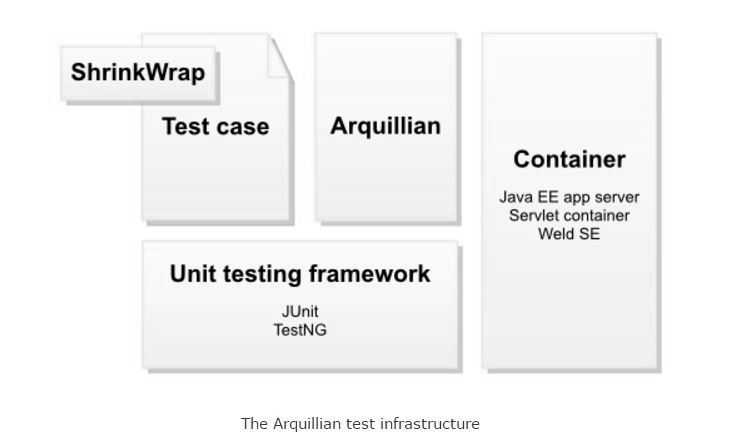
\includegraphics[scale=0.55]{Arquillian.jpg}
	\end{figure}
		
	\vspace{0.5cm}
	\newpage
	Arquillian will be mainly used for:
	\begin{itemize}
		\item Managing the lifecycle of one or more containers
		\item Bundling the test case, dependent classes and resources into a ShrinkWrap archive
		\item Deploying the archive to the container
		\item Enriching the test case by providing dependency injection and other declarative services
		\item Executing the tests inside (or against) the container
		\item Capturing the results and returning them to the test runner for reporting
	\end{itemize}
	
		
	\vspace{0.5cm}
		
	ShrinkWrap is the simplest way to create and define custom archives in Java, that encapsulate the test class and its dependent resources, powering the Arquillian deployment mechanism. In fact, the test case is dispatched to the container's environment through coordination with ShrinkWrap: Arquillian packages the ShrinkWrap-defined archive at runtime and deploys it to the target container.
		
	\subsection{Manual testing.} Manual testing can be considered a valid solution, depending on the application to be tested.\\ In this case a tester ensures the correct behaviors of the components, by following a test plan that allows him to find the most important use cases, without any support from tools or scripts.\\ This is used in alternative of the automated tests, which is more quickly, less expensive and more accurate, because in some particular scenarios it is necessary to exploit human observation, logic and experience.
	\subsection{Maven failsafe (?)}

\newpage
\section{Program	Stubs	and	Test	Data	Required}
	% Based	on	the	testing	strategy	and	test	design,	identify	any	program	stubs or	special	test	data	required	for	each	integration	step.

\end{document}